\chapter{Visual Design}
In order to generate a visual design for the application, different aspects need to be taken into account. On the one hand, the psychological effects of perception are a core aspect, on the other hand the technique of designing a graphical user interface (GUI). The GUI is essential since the credibility judgments of a user over an website or application are based about 75\% on its aesthetics and occur in less than 3.5 seconds \parencite[see.][1]{Alsudani.2009}.
\section{Psychology of Perception}
Due to the GUI being the main interface to the underlying functionality, it is exceptionally important to build an easy to use and easy to understand user interface \parencite[see.][2]{Dray.1995}. In order to build an easy to understand GUI, understanding the foundation of the psychology of perception is essential.
\subsection{Attention Economy}
The topic of \textit{Attention Economy} deals with the scarcity of the ability of people to pay attention. In modern times, one does not only do one thing at work, but is continuously given information  \parencite[see.][]{Davenport.2001}. \textcite{Davenport.2001} state, that for successful transfer of knowledge, understanding attention economy is essential. 
\paragraph*{} \textit{Attention Economy} treats the attention of a person as a limited resource. It is distinguished by the trait of being naturally limited and transient. This means, that a moment not used for paying attention for something is neither able to be restored or savable. \parencite[see.][]{Davenport.2001}
\paragraph*{} The reason for \textit{Attention Economy} to become relevant is the increasing amount of available information. The increasing diversity and density of information caused in the mainstream of digital media and the internet in form of online news, e-mail, social media etc. in addition to traditional communication and information channels such as TV, radio, telephony, letters etc.
\paragraph*{} Derived from that, one can regard attention as a money worth good \parencite[see.][]{Davenport.2001}. While market penetration is narrative for marketing purposes, one must take into account, that potential users of the marketing application may leave the application after a short time in favor of competing consumers of attention.
\subsection{Principles of Perception}
Facing the challenges of \textit{Attention Economy}, business decision makers must explore applications at a higher speed that private users, because as stated above, spend attention implies costs of opportunity \parencite[see.][]{Bakar.2017}. Therefore, designing a application must be done in optimization for fast knowledge transfer and easy exploration. In order to achieve this goal, \textcite{Bakar.2017} suggests a set of goals:
\paragraph*{Getting Started Fast} implies, that no unnecessary contents are disturbing the user from using the core functionality of the page by drastically removing  \say{explanatory and procedural information and let the user learn [...] through exploration} \parencite{Bakar.2017}. 
\paragraph*{Training on Real Tasks} leads the user more easily receiving information and being more restrained by the application, due to a sense of excitement.
\paragraph*{Reading in Any Order} means the quality of the individual information to be not to have perquisite knowledge of any other page within the application.
\paragraph*{Exploiting Prior Knowledge} can help to keep the users attention by mostly presenting new information. This is documented as being dificult to be implemented successfully \sekcite{Carroll.1987}{}{Farkas.1990}{}.
\paragraph*{Coordinating System and Training} represents the progress of novice users in learning to work with the software. This is accomplished by keeping the users attention on the user interface and supplying constructive information.
\paragraph*{Supporting Error Recognition and Recovery} implies strong testing of the application to determine necessary error recognition and implement sufficient information recovery.
\paragraph*{Using the Situation} suggest providing the user many ways to explore the application in means of functionality and informational contents. Offering options for preoccupying oneself with the application amplifies the information transfer but increases the potential for errors.
\paragraph*{Developing Optimal Training Design} pertains the correlation of the user interface design to the users needs and behaviours. 
\paragraph*{Reasoning and Improvising} relatives the approach of explorative interaction by offering instructions where compulsory.
\paragraph*{} Those principles help developers to improve the structural and content wise design of their application, and - as it simplifies the understandability of the application - also the perception of the user, but aesthetic are not directly touched by these. The Gestalt theory describes eight laws for aesthetic designs, which relate to the principle of \textit{Exploiting Prior Knowledge} in terms of using intuitive perceptions of human brains to visually group objects to create a visual composition \parencite[see.][113]{Sternberg.2012}.
\paragraph*{Law of Proximity} Objects that are close to each other, are perceived as mate (see. \ref{fig:prox}). For things to be relatively close to each other, groups must be separated by a larger white space. \parencite{Seogaard.n.y.}
\paragraph*{Law of Similarity} As to be seen in \ref{fig:sim}, objects that share visual properties group themselves visually \\parencite[see.][2]{Bakar.2017}.
\begin{figure}[H] 
    \begin{minipage}[b]{.5\linewidth}
        \centering
\includegraphics[width=0.94\textwidth]{img/proximity.pdf}
        \subcaption{proximity}\label{fig:prox}
    \end{minipage}%
    \begin{minipage}[b]{.5\linewidth}
        \centering
\includegraphics[width=0.94\textwidth]{img/similarity.pdf}
        \subcaption{similarity}\label{fig:sim}
    \end{minipage}
    \caption[Laws of Proximity and Similarity]{Examples of the laws of proximity and similarity (own illustrations)}\label{fig:law1}
\end{figure}
\paragraph*{Law of Closure} Objects that are grouped by visual perception (e.g. by proximity or symmetry) are experienced as a whole (see. \ref{fig:sym}). This principle may suggest objects that are none-existent on the interface \parencite[see.][]{Stevenson.n.y.}.
\paragraph*{Law of Symmetry} Humans tend to perceive objects as two approximate symmetrical halves wherever possible; separate symmetric objects are therefore more likely to be perceived as being one coherent object \parencite[see.][]{Soegaard.n.y.}.
\begin{figure}[H] 
    \begin{minipage}[b]{.5\linewidth}
        \centering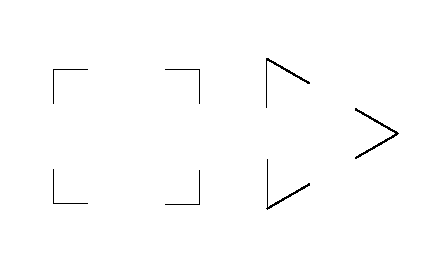
\includegraphics[width=0.94\textwidth]{img/closure.pdf}
        \subcaption{closure}\label{fig:clo}
    \end{minipage}%
    \begin{minipage}[b]{.5\linewidth}
        \centering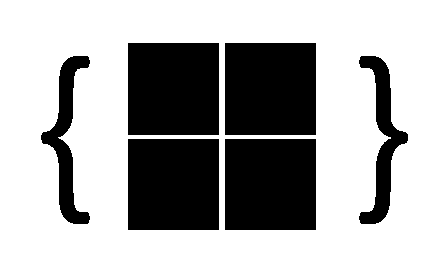
\includegraphics[width=0.94\textwidth]{img/symmetry.pdf}
        \subcaption{symmetry}\label{fig:sym}
    \end{minipage}
    \caption[Laws of Closure and Symmetry]{Examples of the laws of closure and symmetry (own illustrations)}\label{fig:law2}
\end{figure}
\paragraph*{Law of Common Fate} connects objects visually that are moving in the same direction, while separating those fixed in position or moving differently \
\paragraph*{Law of Continuity}
\begin{figure}[H] 
    \begin{minipage}[b]{.5\linewidth}
        \centering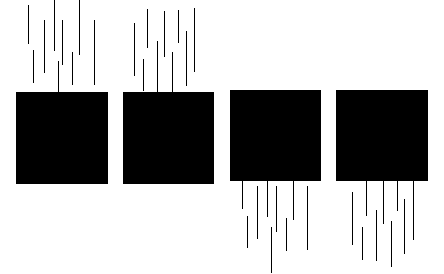
\includegraphics[width=0.94\textwidth]{img/fate.pdf}
        \subcaption{common fate}\label{fig:fate}
    \end{minipage}%
    \begin{minipage}[b]{.5\linewidth}
        \centering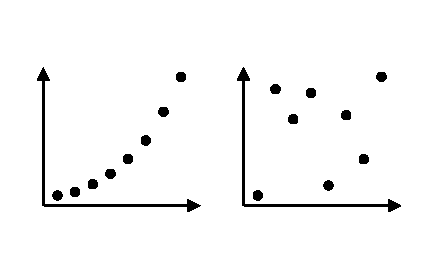
\includegraphics[width=0.94\textwidth]{img/continuity.pdf}
        \subcaption{continuity}\label{fig:con}
    \end{minipage}
    \caption[Laws of Common Fate and Continuity]{Examples of the laws of common fate and continuity (own illustrations)}\label{fig:law3}
\end{figure}
\paragraph*{Law of Good Gestalt}
\paragraph*{Law of Past Experience}\begin{figure}[H] 
    \begin{minipage}[b]{.5\linewidth}
        \centering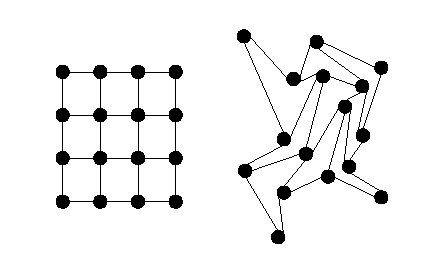
\includegraphics[width=0.94\textwidth]{img/gestalt.pdf}
        \subcaption{good gestalt}\label{fig:gest}
    \end{minipage}%
    \begin{minipage}[b]{.5\linewidth}
        \centering
\includegraphics[width=0.94\textwidth]{img/experience.pdf}
        \subcaption{past experience}\label{fig:exo}
    \end{minipage}
    \caption[Laws of Good Gestalt and Past Experience]{Examples of the laws of good gestalt and past experience (own illustrations)}\label{fig:law4}
\end{figure}
